
In order to demonstrate the efficacy of our proposed algorithm, we undertake a comparative analysis with the performance of Elkan's algorithm, which it extends.
We measure the number of distance evaluations for multiple datasets and for different values of $k$, the number of clusters.
Our implementation is available through GitHub~\cite{Averitchev2024kMeansPtolemy}.

\subsection{Datasets}

\begin{table}[t]
	\centering
	\caption{Datasets used in the experiments}
	\label{tab:datasets}
	\begin{tabular}{llSS}
		\toprule
		\textbf{Group}                                    & \textbf{Dataset}          & \textbf{Cardinality} & \textbf{Dimensionality} \\
		\midrule
		\multirow{2}{*}{\textit{fixed structure}}         & Iris                      & 150                  & 4                       \\
		                                                  & Wine                      & 178                  & 13                      \\
		\cmidrule{2-4}
		\multirow{6}{*}{\textit{variable dimensionality}} & Gaussian Low Dimension    & 10000                & 10                      \\
		                                                  & Gaussian Medium Dimension & 10000                & 100                     \\
		                                                  & Gaussian High Dimension   & 10000                & 300                     \\
		                                                  & Random Low Dimension      & 5000                 & 10                      \\
		                                                  & Random Medium Dimension   & 5000                 & 100                     \\
		                                                  & Random High Dimension     & 5000                 & 300                     \\
		\bottomrule
	\end{tabular}
\end{table}


We employ two groups of datasets to compare the different algorithms, summarized in Table~\ref{tab:datasets}:
The two real-world datasets include the Iris and Wine datasets \cite{pedregosa2011scikit}, which have fixed dimensions and cardinalities and represent different clustering structures.
The two synthetic datasets include Gaussian and uniformly randomly generated points, which are used to test for the effects of changing dataset dimensionality.

\subsection{Experiments}
\todo{If we claim to have implemented the classic k-means, we also have to show that in our plots.}
Our variant of the k-Means algorithm is tested by implementing the classical k-Means algorithm (Lloyd's algorithm), Elkan's algorithm, and its novel, Ptolemy-based extension in Python.

To provide a fair comparison of the algorithms,
we measure the number of distance calculations instead of wall-clock time.
As distance calculations account for the majority of computing time in k-Means algorithms, they offer a clear measure of efficiency regardless of implementational optimizations.

Additionally, two intermediate variants were implemented to assess the separate effects of the lower and upper bounds:
\emph{Ptolemy\_upper} one uses Elkan's lower bound with Ptolemy's upper bound, and \emph{Ptolemy\_lower} uses Ptolemy's lower bound with Elkan's upper bound.

Each algorithm is executed three times on each dataset, with the parameters $k = 3$, $k = 20$, and $k = 100$.

In \autoref{fig:combined}, we report our results as distance calculations saved relative to Elkan's algorithm, showcasing any improvements introduced by the proposed extension.

%The experiments evaluate the algorithms based on the number of distance calculations, which dominate the computing time in k-Means algorithms. This metric ensures comparability across different implementations and hardware setups. 


\subsection{Discussion}

\begin{figure}[h]
	\centering
	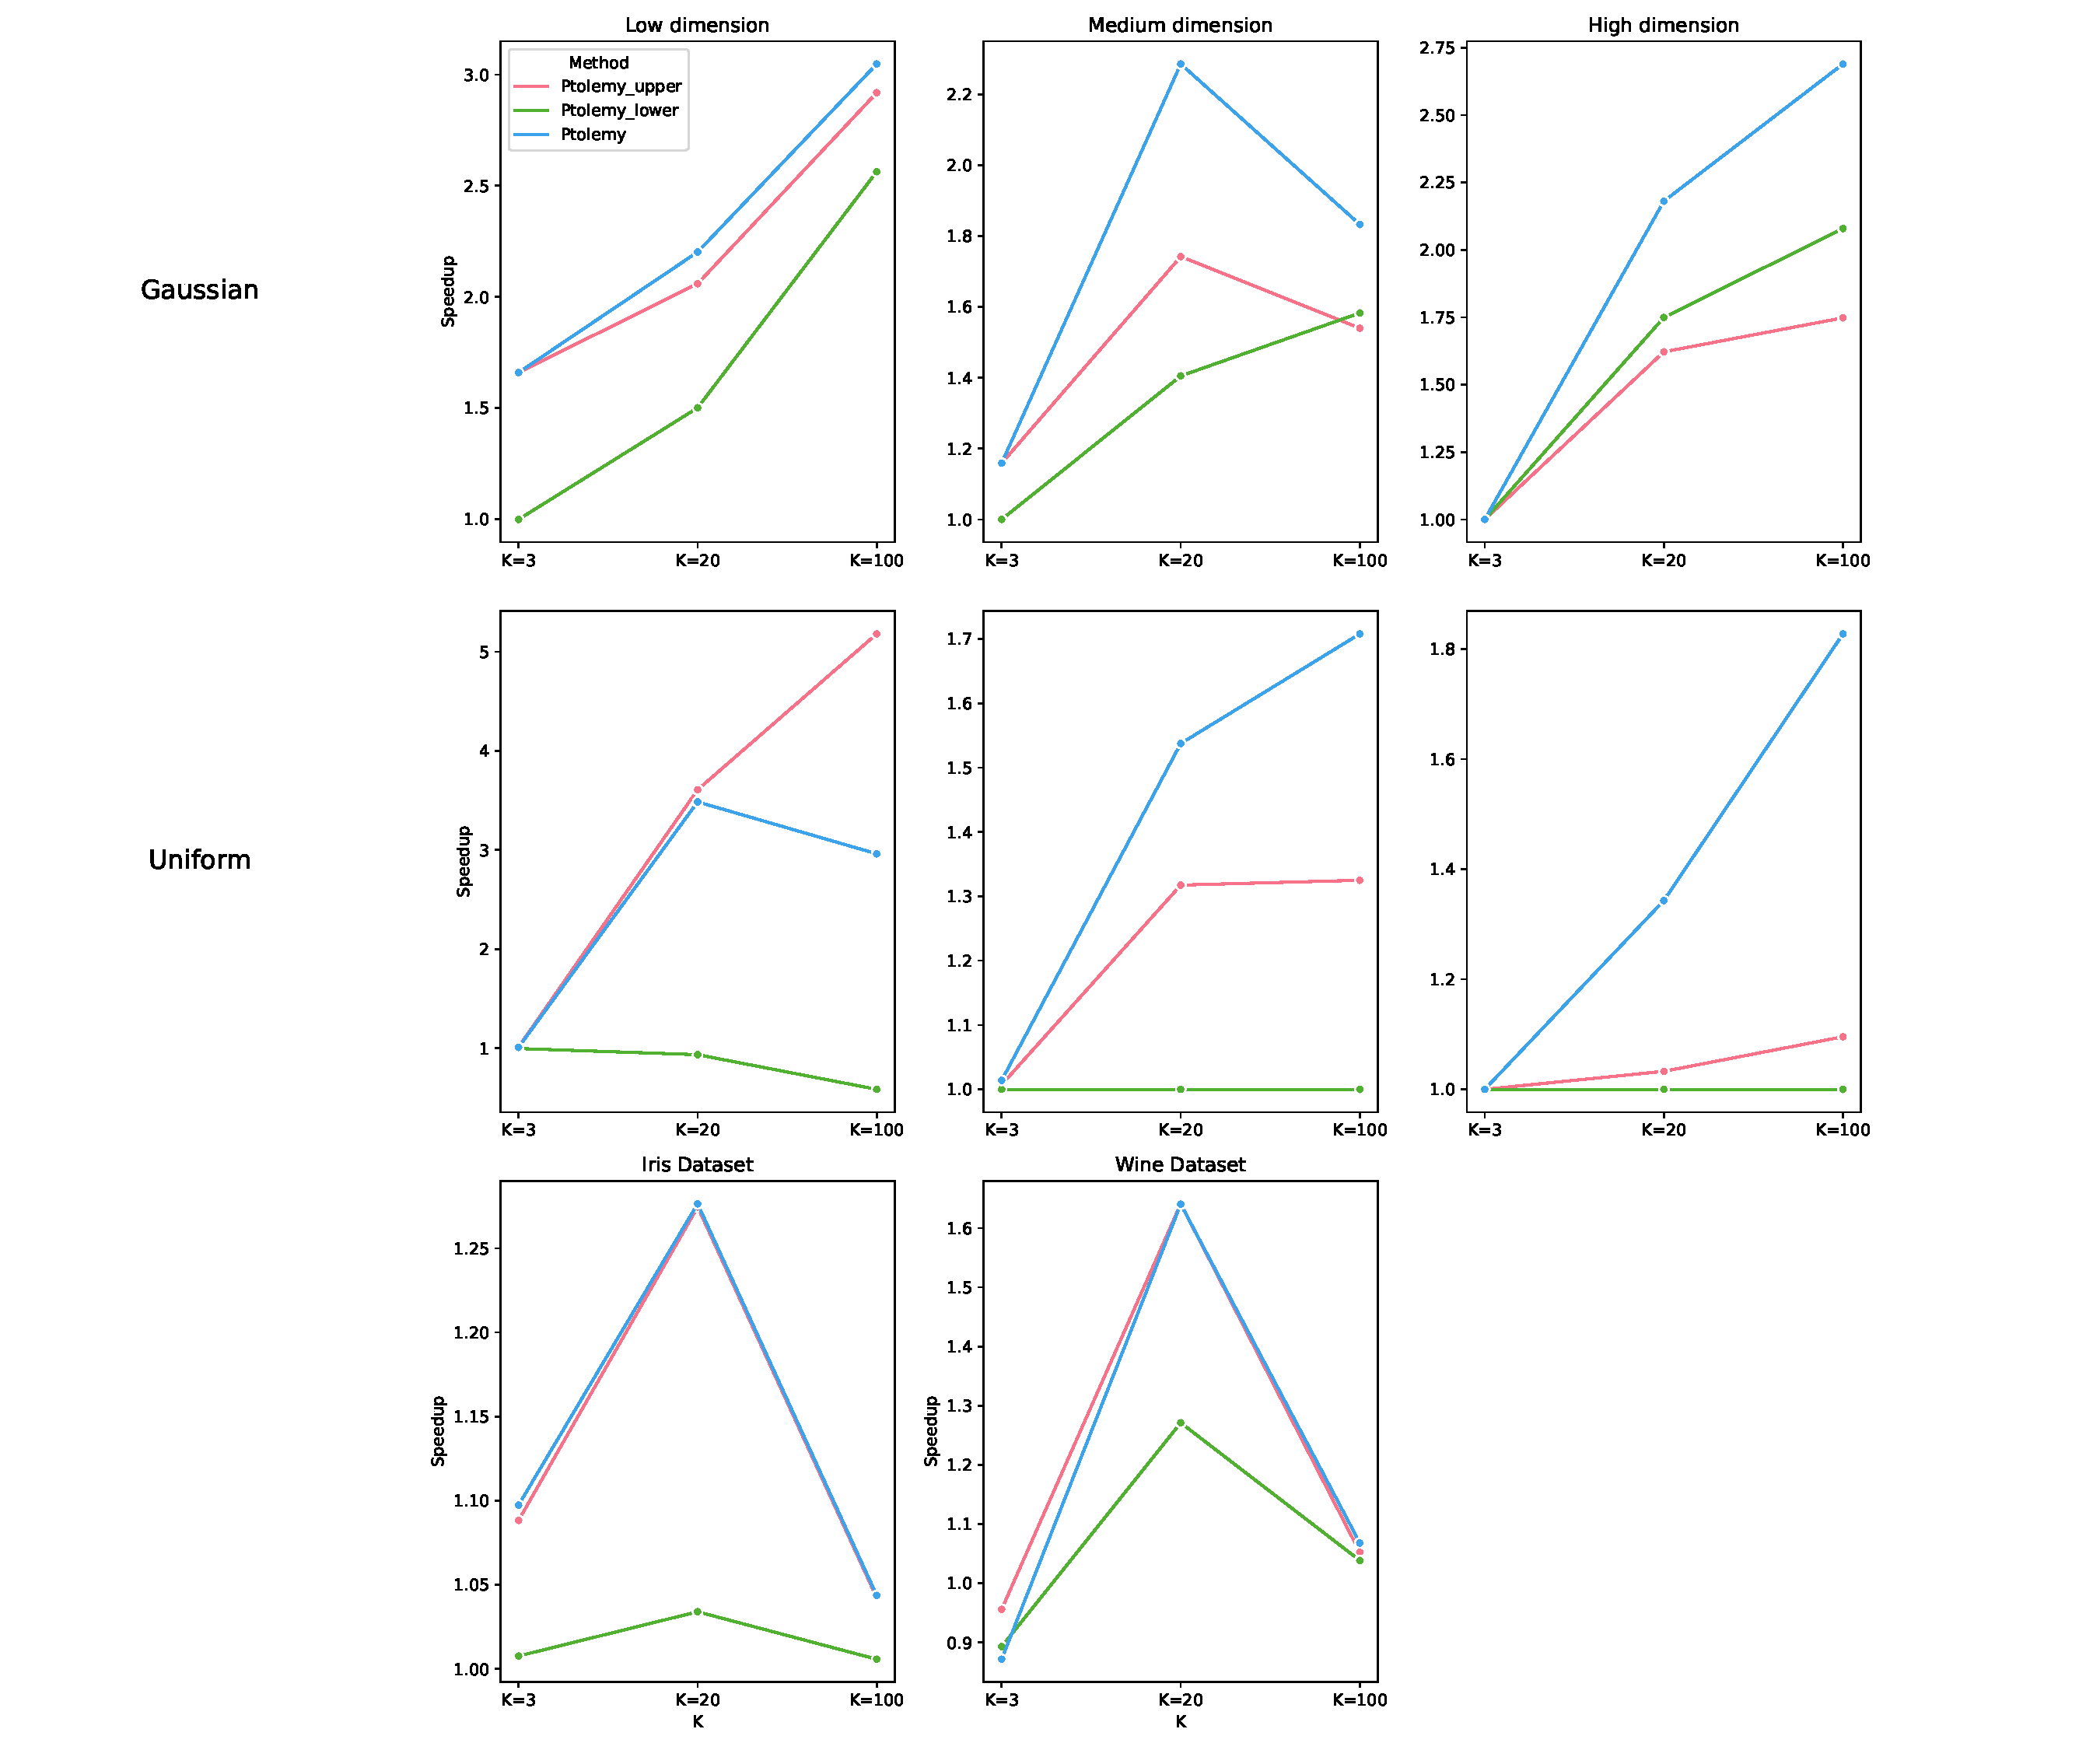
\includegraphics[width=\textwidth]{fig/combined_plot.pdf}
	\caption{
		Relative number of saved distance evaluations, compared to Elkan's algorithm.
		Top and middle row: Performance increases on synthetic data generated from Gaussian (top) and uniformly random (middle) distributions.
		The dimensionality of the dataset increases left-to-right.\\
		Bottom row: Performance increases on the real-world datasets Iris (left) and Wine (right).
	}
	\label{fig:combined}
\end{figure}


The primary focus of this analysis is the full Ptolemaic algorithm, as it is the most robust when comparison to Elkan's algorithm.
In general, the full Ptolemaic extension shows substantial improvements in reducing the number of distance evaluations across most scenarios.

\textbf{Number of Clusters.}
The full Ptolemaic algorithm consistently demonstrates significant improvements over Elkan’s algorithm as the number of clusters $k$ increases.
For instance, in the Gaussian low-dimensional dataset, the Ptolemaic algorithm achieves larger than 2-fold speedups for $k = 20$ and $k = 100$, illustrating its ability to significantly reduce distance calculations in complex clustering tasks.
% surpasses 3-fold improvements for
% Similar trends are observed in the Random low-dimensional dataset.
For smaller cluster counts ($k = 3$), the advantage is less pronounced, with speedups around 1.1 in the Iris and Wine datasets.
This suggests that Ptolemy's inequality offers significant improvements for larger values of $k$.
However, lower-complexity clustering tasks may not benefit to the same extent,
given the additional overhead imposed by the Ptolemaic bounds, which are computationally more complex to evaluate compared to the triangle bounds.
The Ptolemaic Upper Bound variant performs comparably to the full Ptolemaic algorithm, especially for larger $k$ values.
However, the Lower Bound variant underperforms in some cases, particularly with smaller cluster counts or in higher-dimensional datasets.

\textbf{Dimensionality.} The full Ptolemaic algorithm performs well across varying dimensionality. In low-dimensional datasets (10 dimensions), it achieves impressive speedups, particularly at higher cluster counts.
As dimensionality increases, performance gains persist but become slightly less pronounced.
Nonetheless, even in higher-dimensional datasets, the full Ptolemaic algorithm remains effective, consistently reducing distance evaluations.
However, the Ptolemaic lower bound variant often struggles in these higher-dimensional cases, further emphasizing the robustness of the full Ptolemaic approach.

% \textbf{Summary.}
% The full Ptolemaic algorithm demonstrates consistent and significant improvements over Elkan’s algorithm across a variety of datasets.
% In particularly at a high number of clusters and low to medium dimensionality.
% The Ptolemaic upper bound variant performs similarly in many cases, offering comparable efficiency gains, whereas the Ptolemaic lower bound variant, particularly in datasets with higher dimensionality or smaller cluster counts. Overall, the full Ptolemaic algorithm proves to be a robust and efficient alternative to traditional k-Means implementations, especially as the complexity of the clustering task increases.


\textbf{Limitations.}
The presented experiments are subject to three primary constraints:
(i) While synthetic random datasets provide valuable best-case scenarios, more extensive real-world data with appropriate grouping structures is necessary for comprehensive evaluation.
(ii) The significant reduction in distance calculations may not directly translate to improved execution times, as Ptolemy's bounds are computationally more expensive than the triangle inequality.
(iii) Most critically, the limited sample size and fixed initial conditions, particularly the lack of variation in cluster initializations, severely restrict the generalizability of individual measurements.\\
Despite these limitations, we contend that the observed overall trend remains compelling and warrants further investigation into the application of Ptolemy's inequality for clustering algorithms.

% The experiments presented suffer from two main factors:
% - minor caveat: synthetic random datasets are good worst-case scenarios, but larger amounts of real-world data is needed.
% - major caveat: sample size and initial conditions. experiments don't vary cluster initializations. while the results presented aren't cherry-picked, single measurements contain only little information.
% - despite these shortcommings, we believe that the overall trend is still convincing.

% The experimental results, presented in the figures, provide critical insights into the performance of the k-Means algorithm variants. The primary focus of this analysis is on the full Ptolemaic algorithm and its comparison with Elkan’s algorithm. The results highlight several scenarios in which the full Ptolemaic algorithm achieves substantial improvements over Elkan’s approach, particularly in reducing the number of distance evaluations.
%
% \textbf{Number of Clusters.} The full Ptolemaic algorithm consistently demonstrates notable improvements over Elkan’s algorithm as the number of clusters ($k$) increases. For instance, in the Gaussian low-dimensional dataset, the Ptolemaic algorithm achieves speedups of over 2-fold for $k = 20$ and surpasses 3-fold for $k = 100$, illustrating its ability to significantly reduce distance calculations in more complex clustering tasks. Similar trends are observed in the Random low-dimensional dataset, where the full Ptolemaic algorithm achieves a speedup of more than 3-fold at $k = 20$ and $k = 100$. These results underscore the increasing efficiency of the Ptolemaic algorithm as the clustering complexity grows.
%
% In contrast, for smaller cluster counts, such as $k = 3$, the performance advantage of the full Ptolemaic algorithm is less pronounced but still evident, with speedups of around 1.1 in both the Iris and Wine datasets. This suggests that while Ptolemy’s inequality offers significant improvements for larger $k$ values, it still provides moderate gains for smaller cluster sizes.
%
% The Ptolemaic Upper Bound variant performs comparably to the full Ptolemaic algorithm, especially for larger $k$ values, delivering similar efficiency improvements. However, the Ptolemaic Lower Bound variant tends to underperform in some cases, particularly with smaller cluster counts or in higher-dimensional datasets, where its speedup is sometimes close to or even below that of Elkan’s algorithm.
%
% \textbf{Dimensionality.} The full Ptolemaic algorithm also performs well across datasets with varying dimensionality. In the Gaussian low-dimensional dataset (10 dimensions), the full Ptolemaic algorithm achieves impressive speedups, particularly at higher cluster counts, with speedups over 3-fold at $k = 100$. As the dimensionality increases, the performance gains of the Ptolemaic algorithm persist, though they become slightly less pronounced. For example, in the Gaussian medium (100 dimensions) and Gaussian high (300 dimensions) datasets, the Ptolemaic algorithm continues to offer significant speedups, but the performance advantage over Elkan’s algorithm decreases slightly.
%
% In higher-dimensional datasets, such as the Random high-dimensional dataset, the full Ptolemaic algorithm remains effective, consistently reducing the number of distance evaluations, particularly for larger $k$ values. However, the Ptolemaic Lower Bound variant often struggles in these higher-dimensional cases, further emphasizing the robustness of the full Ptolemaic approach.
%
% \textbf{Summary.} The full Ptolemaic algorithm demonstrates consistent and significant improvements over Elkan’s algorithm across a variety of datasets, particularly in scenarios with a high number of clusters and low to medium dimensionality. The Ptolemaic Upper Bound variant performs similarly in many cases, offering comparable efficiency gains, whereas the Ptolemaic Lower Bound variant sometimes struggles, particularly in datasets with higher dimensionality or smaller cluster counts. Overall, the full Ptolemaic algorithm proves to be a robust and efficient alternative to traditional k-Means implementations, especially as the complexity of the clustering task increases.
